\section{Juridinis įgyvendinamumas}

Kuriama sistema neprieštarauja Lietuvos Respublikos įstatymams. Stovyklos 
dalyvių asmens duomenų rinkimas neprieštarauja Lietuvos Respublikos 
Asmens duomenų teisinės apsaugos įstatymui. Kiekvienam dalyviui bus 
suteikiama galimybė nesutikti su jo asmens duomenų rinkimu, arba davus 
leidimą peržiūrėti jau surinktus duomenis ir panorėjus juos pakeisti. 
Pasibaigus stovyklos organizavimo ir vykdymo laikotarpiui nereikalingi 
duomenys bus sunaikinami. Taip pat numatoma laikytis visų duomenų saugumo 
kriterijų.
% TODO Pridėti nuorodą į straipsnį.

\section{Sistemos panaudojimas}

\ref{fig:uml_tasks} UML schemoje vaizduojamos aktorių vykdomos užduotys ir 
kaip jas padeda vykdyti sistema.

\begin{figure}[htb]
  \begin{center}
    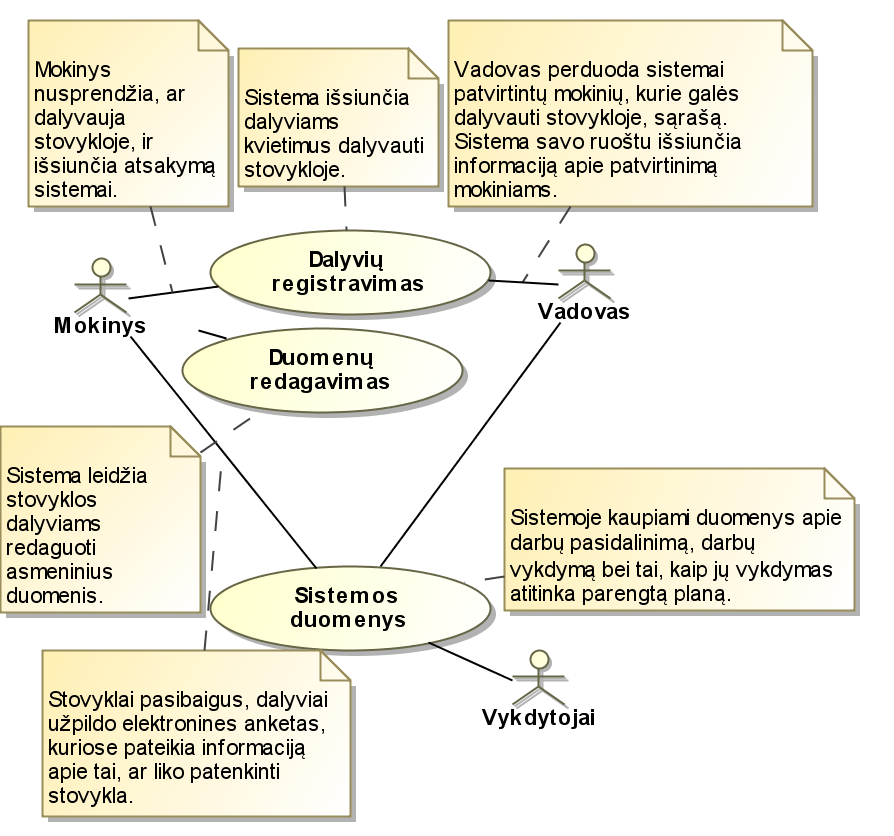
\includegraphics[scale=0.8]{images/sistemos_panaudojimas.png}
  \end{center}
  \caption{UML schema vaizduojamos aktorių vykdomos užduotys ir kaip jas
    padeda vykdyti sistema.}
  \label{fig:uml_tasks}
\end{figure}

\section{Sistemos teikiama nauda}

\ref{fig:uml_tasks2} UML schema vaizduojamos aktorių vykdomos užduotys 
ir kaip jas
padeda vykdyti sistema.

\begin{figure}[htb]
  \begin{center}
    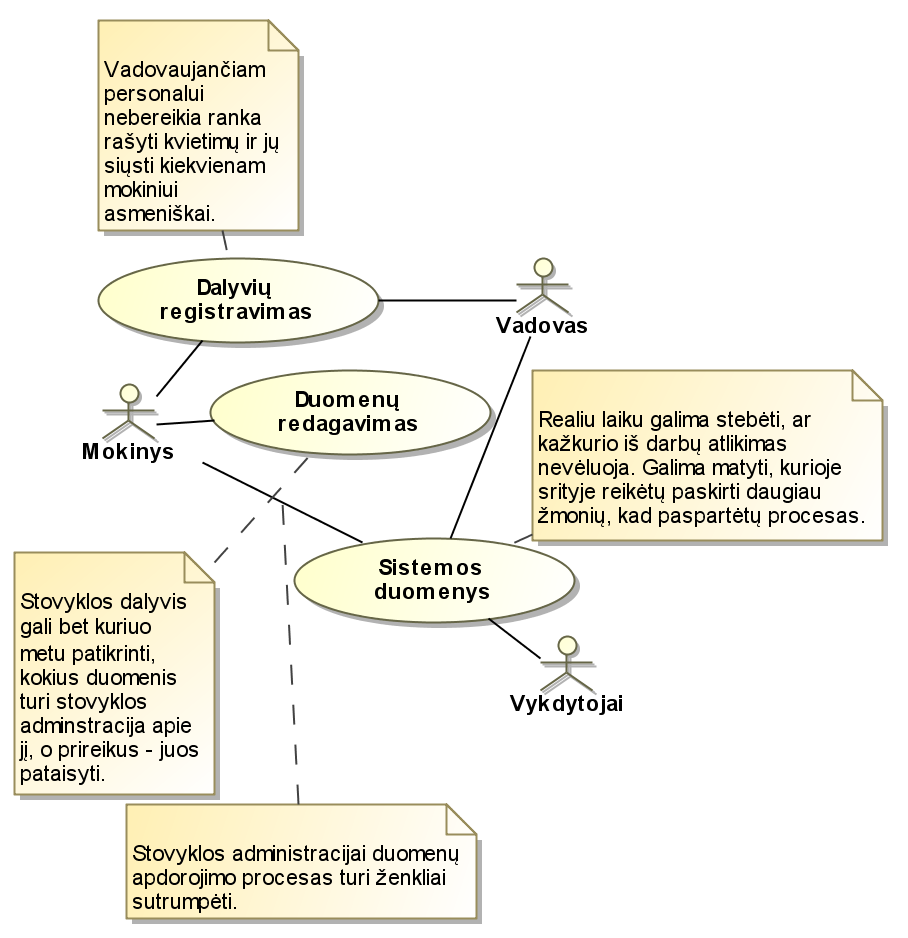
\includegraphics[scale=0.8]{images/sistemos_tiekiama_nauda.png}
  \end{center}
  \caption{UML schema vaizduojamos aktorių vykdomos užduotys ir kaip jas
    padeda vykdyti sistema.}
  \label{fig:uml_tasks2}
\end{figure}
